\documentclass[11pt,reqno]{amsart}

\usepackage[T1]{fontenc}
\usepackage{lmodern}
\usepackage[utf8]{inputenc}
\usepackage{amsmath,amssymb,amsthm,mathtools}
\usepackage{bm}
\usepackage{booktabs}
\usepackage{array}
\usepackage{graphicx}
\usepackage{xcolor}
\usepackage{enumitem}
\usepackage[margin=1.12in]{geometry}
\usepackage{microtype}
\usepackage[hypertexnames=false]{hyperref}
\usepackage{cleveref}

\definecolor{acadblue}{rgb}{0.05,0.22,0.55}
\emergencystretch=1.8em

\hypersetup{
  colorlinks=true,
  linkcolor=acadblue,
  citecolor=acadblue,
  urlcolor=acadblue,
  pdftitle={Combinatorial Euler-Sieve Identities, Hadamard-Poisson Flux Detection, and Conditional Nodal-Wall Identities for Riemann's Xi-Function},
  pdfauthor={Thijs Missiaen}
}

\theoremstyle{plain}
\newtheorem{theorem}{Theorem}[section]
\newtheorem{proposition}[theorem]{Proposition}
\newtheorem{lemma}[theorem]{Lemma}
\newtheorem{corollary}[theorem]{Corollary}

\theoremstyle{definition}
\newtheorem{definition}[theorem]{Definition}

\theoremstyle{remark}
\newtheorem{remark}[theorem]{Remark}

\numberwithin{equation}{section}

\newcommand{\dd}{\,\mathrm{d}}
\newcommand{\ii}{\mathrm{i}}
\newcommand{\ee}{\mathrm{e}}
\newcommand{\fac}{\mathclose{\mathchar"0021}}
\DeclareMathOperator{\Reop}{Re}
\DeclareMathOperator{\Imop}{Im}
\DeclareMathOperator{\sgn}{sgn}

\title[Euler-Sieve Identities, Hadamard Flux Detection, and Nodal Walls]{Combinatorial Euler-Sieve Identities, Hadamard--Poisson Flux Detection,\\ and Conditional Nodal-Wall Identities for Riemann's $\Xi$-Function}

\author{Thijs Missiaen}
\address{Independent Researcher, Belgium \\ ORCID: \href{https://orcid.org/0009-0007-3678-0810}{0009-0007-3678-0810}}
\email{thijs.missiaen@gmail.com}
\date{October 2026 (Revised Audit Edition)}
\subjclass[2020]{Primary 11M06, 11M26; Secondary 30D15, 46C20}
\keywords{Riemann $\Xi$-function, Euler-sieve Dirichlet coefficients, Kronecker density, Voronin universality, Hadamard--Poisson flux, Lagarias positivity, de Branges Gram matrix, nodal curves}

\begin{document}

\begin{abstract}
We analyze three constructions for Riemann's completed zeta function $\Xi(t - \ii d) := \xi(\frac{1}{2} + d + \ii t)$ and its canonical transverse Wronskian $W(d,t) := \frac{1}{2}\partial_d\lvert\Xi(t - \ii d)\rvert^2 = 16\int_0^\infty y\sinh(2dy)I(y,t)\dd y$, separating exact identities from structural obstructions. First, we prove the finite cubic-window Dirichlet identity for $\zeta(s)\prod_{p \le X}(1 - p^{-s})$ on $1 \le N < (\lfloor X\rfloor + 1)^3$, while showing that $F_2(z) = 1 + z + \frac{1}{2}z^2$ vanishes at $z = -1 \pm \ii$, $\mathcal{P}_{>X}(s)$ diverges in $0 < \sigma \le 1$, and Kronecker density on small primes produces arbitrary complex excursions. Second, we evaluate the Poisson--Hadamard lobe integral $\mathcal{F}_-(d, d_*) = -\arcsin(d/d_*)$ and Sylvester inertia jump on a pole-free entire two-zero perturbation as contrapositives of Lagarias's equivalence. Third, we formulate the Cauchy--Riemann nodal-wall identity along $I(d, \tau(d)) = 0$ with explicit non-circularity hypotheses and contrast Jacobi's $\vartheta_3(0 \mid \ii\ee^{4u}) \neq 0$ with the imaginary root $\Phi(\ii\eta_0) = 0$ at $\eta_0 = 0.319415\dots < \frac{\pi}{8}$.
\end{abstract}

\maketitle

\section{Introduction}\label{sec:intro}

Let $\Xi(t - \ii d) := \xi(\frac{1}{2} + d + \ii t) = R(d,t) + \ii I(d,t)$ denote Riemann's completed zeta function at $s = \frac{1}{2} + d + \ii t$~\cite{riemann1859,titchmarsh1986}, represented by the even Jacobi-theta integral
\begin{equation}\label{eq:xi_def}
\Xi(t - \ii d) = 8\int_0^{\infty} \Phi(u)\cos\!\bigl(2(t - \ii d)u\bigr)\dd u, \qquad \Phi(u) := \sum_{n=1}^{\infty} \bigl(2\pi^2 n^4\ee^{9u} - 3\pi n^2\ee^{5u}\bigr)\ee^{-\pi n^2\ee^{4u}}.
\end{equation}
In our canonical normalization across this series, the transverse Wronskian and its desingularized quotient $\widetilde{W}(d,t) := W(d,t)/d$ are given by
\begin{equation}\label{eq:canonical_W}
W(d,t) := \frac{1}{2}\frac{\partial}{\partial d}\bigl\lvert\Xi(t - \ii d)\bigr\rvert^2 = R\partial_d R + I\partial_d I = 16\int_0^{\infty} y\sinh(2dy)\,I(y,t)\dd y,
\end{equation}
where $I(y,t) := \int_{-\infty}^{\infty}\Phi(\frac{y+x}{2})\Phi(\frac{y-x}{2})\cos(2tx)\dd x$ is the Wigner-type autocorrelation along $y = u + v$, $x = u - v$~\cite{wigner1932,hudson1974}. Classical function-theoretic criteria due to Speiser~\cite{speiser1934}, Jensen~\cite{jensen1913}, P\'olya~\cite{polya1926}, de~Branges~\cite{debranges1968}, Hinkkanen~\cite{hinkkanen1997}, and Lagarias~\cite{lagarias1999} reformulate the Riemann Hypothesis in terms of the positivity of $\Reop(\xi'(s)/\xi(s))$ on $d > 0$ or the positive semi-definiteness of de~Branges reproducing-kernel Gram matrices in the lower half-plane $z = t - \ii d$ ($d > 0$).

When studying these positivity structures alongside Euler-product sieves and level curves of $\Xi$ (the X-ray geometry investigated by Speiser~\cite{speiser1934} and Arias de Reyna~\cite{ariasdereyna2003}), three subtle pitfalls arise if formal or local identities are extrapolated beyond their domain of validity: (i) confusing formal exponential Dirichlet-series identities on $\sigma > 1$ or real-slice polynomial floors with complex strip bounds in the presence of Kronecker phase density; (ii) mistaking contrapositive zero-detection signatures of an assumed off-critical zero for unconditional zero-prevention theorems; and (iii) assuming global smoothness or non-vanishing along nodal curves $I(d,\tau(d)) = 0$ without checking critical points $\Xi'(z_c) = 0$ or zeros of $\Phi(u)$ in the complex $u$-strip. This paper establishes the exact identities that hold in each setting together with explicit counterexamples delineating their analytical boundaries.

\subsection{Proof overview}\label{subsec:overview}

The paper is organized into three main analytical sections:
\begin{enumerate}[label=\textup{(\arabic*)},leftmargin=2.2em]
\item \textbf{Cubic-window Dirichlet identity versus complex roots of $F_2$, strip divergence, and Kronecker alignment (\Cref{sec:cubic}).} \Cref{prop:cubic_window} proves the exact combinatorial identity expressing the Dirichlet coefficients $b_N^{\mathcal{E}}(X)$ of $\zeta(s)E_X(s)$ on the cubic window $1 \le N < (\lfloor X\rfloor + 1)^3$ via the quadratic truncation $1 + \mathcal{P}_{>X} + \frac{1}{2}\mathcal{P}_{>X}^2$ as formal Dirichlet series (and analytically for $\sigma > 1$). \Cref{prop:kronecker_obstruction} then proves three sharp obstructions: while $\lvert F_2(U,0)\rvert^2 = \frac{1}{4}((1+U)^2+1)^2 \ge \frac{1}{4}$ holds along the real line $V = 0$, $F_2(z) = 1 + z + \frac{1}{2}z^2$ vanishes in $\mathbb{C}$ at $z = -1 \pm \ii$; the prime Dirichlet series $\mathcal{P}_{>X}(s)$ diverges throughout $0 < \sigma \le 1$; and astronomically long simultaneous recurrence times on all $\pi(N(t))$ primes do \emph{not} prevent destructive alignment, because Kronecker's theorem on a fixed finite subset of small primes already drives finite prime sums arbitrarily close to $-1 \pm \ii$ (in accord with Bohr--Landau~\cite{bohrlandau1914}, Voronin~\cite{voronin1975}, and Montgomery~\cite{montgomery1977}).
\item \textbf{Closed-form Poisson--Hadamard lobe integral and pole-free de Branges inertia jump (\Cref{sec:flux}).} \Cref{thm:hadamard_flux} proves in closed form that the single-pair Poisson--Hadamard kernel of an off-critical quadruple $\pm\gamma_* \pm \ii d_*$ ($d_* > 0$) has negative central lobe integral $\mathcal{F}_-(d, d_*) = -\arcsin(d/d_*)$ for $0 < d < d_*$ and total step $\mathcal{F}(d, d_*) = \pi\Theta(d - d_*)$. \Cref{prop:gram_detection} evaluates the corresponding Sylvester negative inertia jump $\nu_-(\mathbf{G}_\alpha(d)) \ge 1$ on an explicit \emph{pole-free} entire even two-zero coalescence perturbation $\Xi_{\mathrm{pert}}(z; d_*)$ (correcting singular rational test factors that create poles at simple zeros). Both results are framed accurately as contrapositives of Lagarias's~\cite{lagarias1999} equivalence: they detect off-critical zeros (including those of the Davenport--Heilbronn function~\cite{davenportheilbronn1936}) rather than preventing them.
\item \textbf{Conditional nodal-wall identity and the pure-imaginary zero of $\Phi$ (\Cref{sec:chladni}).} \Cref{prop:nodal_wall} derives the local Cauchy--Riemann identity $\widetilde{W}(d,\tau(d)) = R(d,\tau(d))\partial_t I(d,\tau(d))/d$ along a smooth branch $I(d,\tau(d)) = 0$, isolating the three explicit hypotheses required for positivity and constructing an explicit polynomial counterexample $Q(z)$ satisfying $-Q(\tau_0)Q''(\tau_0) > 0$ at $d = 0$ that nevertheless vanishes on its own $I = 0$ curve at $d = d_*$. Finally, \Cref{prop:phi_zero} contrasts Jacobi's triple-product non-vanishing $\vartheta_3(0 \mid \ii\ee^{4u}) \neq 0$ on $\lvert\Imop(u)\rvert < \frac{\pi}{8}$ with the explicit pure-imaginary zero $\Phi(\ii\eta_0) = 0$ at $\eta_0 = 0.3194150268\dots < \frac{\pi}{8}$, demonstrating that differential operators do not preserve strip zero-freeness.
\end{enumerate}

\subsection{Notation and conventions}\label{subsec:notation}

Throughout, $s = \sigma + \ii t = \frac{1}{2} + d + \ii t$ with $d = \sigma - \frac{1}{2} \ge 0$, $z = t - \ii d \in \mathbb{C}$, and $\Xi(z) = \xi(\frac{1}{2} + \ii z) = R(d,t) + \ii I(d,t)$. Note that Cauchy--Riemann differentiation of $\Xi(t - \ii d)$ yields $\partial_d R(d,t) = \partial_t I(d,t)$ and $\partial_d I(d,t) = -\partial_t R(d,t)$. For $X \ge 2$, $E_X(s) := \prod_{p \le X}(1 - p^{-s})$, and $\zeta(s)E_X(s) = \sum_{N=1}^{\infty} b_N^{\mathcal{E}}(X)N^{-s}$ ($\sigma > 1$). We denote by $0 < \gamma_1 < \gamma_2 < \dots$ the positive critical-line zeros of $\Xi(t)$ ($\gamma_1 = 14.13472514\dots$, $\gamma_2 = 21.02203964\dots$).

\section{Combinatorial Cubic-Window Identity and Small-Prime Alignment Obstructions}\label{sec:cubic}

For $\sigma > 1$, Euler's product formula gives $\zeta(s)E_X(s) = \prod_{p > X}(1 - p^{-s})^{-1} = \exp(\mathcal{P}_{>X}(s))$, where the sieved prime-power Dirichlet series is
\begin{equation}\label{eq:prime_dirichlet}
\mathcal{P}_{>X}(s) := \sum_{n=2}^{\infty} c_n(X)\,n^{-s} = \sum_{p > X}\sum_{r=1}^{\infty} \frac{1}{r}\,p^{-rs}, \qquad c_n(X) := \begin{cases} \dfrac{1}{r} & \text{if } n = p^r \text{ with } p > X, \\[4pt] 0 & \text{otherwise.} \end{cases}
\end{equation}

\begin{proposition}[Combinatorial cubic-window Dirichlet identity]\label{prop:cubic_window}
Let $X \ge 2$, and expand $\exp(\mathcal{P}_{>X}(s)) = \sum_{k=0}^{\infty}\frac{1}{k\fac}(\mathcal{P}_{>X}(s))^k$ as a formal Dirichlet series (or as an absolutely convergent Dirichlet series on $\sigma > 1$). For every integer $N$ in the cubic window $1 \le N < (\lfloor X\rfloor + 1)^3$, all terms with $k \ge 3$ contribute zero to the coefficient of $N^{-s}$, so
\begin{equation}\label{eq:cubic_coeff}
b_N^{\mathcal{E}}(X) = \delta_{N,1} + c_N(X) + \frac{1}{2}\sum_{\substack{d \mid N \\ 2 \le d \le N/2}} c_d(X)\,c_{N/d}(X) \qquad \bigl(1 \le N < (\lfloor X\rfloor + 1)^3\bigr).
\end{equation}
\end{proposition}

\begin{proof}
The Dirichlet series $\mathcal{P}_{>X}(s)$ is supported on integers $n \ge \lfloor X\rfloor + 1$. Consequently, for every $k \ge 3$, the $k$-fold Dirichlet convolution $(\mathcal{P}_{>X}(s))^k$ is supported on integers $N = n_1 \cdots n_k \ge (\lfloor X\rfloor + 1)^k \ge (\lfloor X\rfloor + 1)^3$. By uniqueness of formal Dirichlet coefficients (equivalently, uniqueness on $\sigma > 1$), matching coefficients of $N^{-s}$ in $\zeta(s)E_X(s) = \sum_{k=0}^{\infty} \frac{1}{k\fac}\mathcal{P}_{>X}(s)^k$ for $1 \le N < (\lfloor X\rfloor + 1)^3$ retains only $k \in \{0, 1, 2\}$, proving~\eqref{eq:cubic_coeff}.
\end{proof}

We now examine the quadratic polynomial $F_2(z) := 1 + z + \frac{1}{2}z^2$ ($z = U + \ii V \in \mathbb{C}$) suggested by~\eqref{eq:cubic_coeff} and establish why neither $F_2$ nor simultaneous Bohr--Kronecker recurrence times can prevent zeros or small values in $0 < \sigma \le 1$.

\begin{proposition}[Complex zeros of $F_2$, strip divergence, and Kronecker small-prime alignment]\label{prop:kronecker_obstruction}
Let $F_2(z) := 1 + z + \frac{1}{2}z^2$ for $z = U + \ii V \in \mathbb{C}$. Then:
\begin{enumerate}[label=\textup{(\roman*)},leftmargin=2.2em]
\item \textbf{Real-slice quadratic minimum versus complex zeros.} Completing the square gives $F_2(z) = \frac{1}{2}[(z + 1)^2 + 1]$, whence
\begin{equation}\label{eq:F2_modulus}
\bigl\lvert F_2(U + \ii V)\bigr\rvert^2 = \frac{1}{4}\Bigl[\bigl((1 + U)^2 + 1 - V^2\bigr)^2 + 4V^2(1 + U)^2\Bigr].
\end{equation}
Along the real axis $V = 0$,~\eqref{eq:F2_modulus} reduces to the elementary quadratic floor $\lvert F_2(U)\rvert^2 = \frac{1}{4}((1+U)^2 + 1)^2 \ge \frac{1}{4}$ (attained at $U = -1$). In the complex plane, however, $F_2(z)$ vanishes identically at the conjugate pair $z = -1 \pm \ii$, i.e.\ $(U, V) = (-1, \pm 1)$.
\item \textbf{Divergence of $\mathcal{P}_{>X}(s)$ in the critical strip.} For every finite $X \ge 2$, the Dirichlet series~\eqref{eq:prime_dirichlet} has abscissa of absolute convergence $\sigma_a = 1$ and diverges at $s = 1$; moreover, $\ln[\zeta(s)E_X(s)]$ has logarithmic branch-point singularities at $s = 1$ and at every zero $\rho$ of $\zeta(s)$ in $0 < \sigma < 1$, so $\mathcal{P}_{>X}(s)$ cannot converge across any half-plane $\sigma > \sigma_0$ containing $1$ or a zero of $\zeta(s)$.
\item \textbf{Failure of simultaneous Kronecker recurrence arguments.} Let $\sigma \in (\frac{1}{2}, 1]$ and $X \ge 2$. Because $\sum_{p > X} p^{-\sigma} = +\infty$, one can choose a fixed finite set of $K$ primes $X < p_1 < \dots < p_K$ such that $\sum_{j=1}^K p_j^{-\sigma} > \sqrt{2} = \lvert -1 + \ii\rvert$ and $p_1^{-\sigma} < \sum_{j=2}^K p_j^{-\sigma} + \sqrt{2}$ (in fact $p_j^{-\sigma} < 1 < \sqrt{2}$). By linear independence of $\{\ln p_1, \dots, \ln p_K\}$ over $\mathbb{Q}$ and Kronecker's theorem on $\mathbb{T}^K$, for every $\varepsilon > 0$ there exist infinitely many $t > 0$ at which the finite prime sum $\mathcal{P}_{X < p \le p_K}(\sigma + \ii t) := \sum_{j=1}^K p_j^{-\sigma - \ii t}$ satisfies $\lvert\mathcal{P}_{X < p \le p_K}(\sigma + \ii t) - (-1 - \ii)\rvert < \varepsilon$ and hence $\lvert F_2(\mathcal{P}_{X < p \le p_K}(\sigma + \ii t))\rvert < \varepsilon$.
\end{enumerate}
\end{proposition}

\begin{proof}
Part~(i) follows directly by expanding $\lvert\frac{1}{2}((U + 1 + \ii V)^2 + 1)\rvert^2$; setting $(z + 1)^2 = -1$ gives $z = -1 \pm \ii$. Part~(ii) is classical: $\sum_{p > X} p^{-1} = +\infty$ by Euler and Mertens, and any convergent Dirichlet series defines a holomorphic function in a half-plane $\sigma > \sigma_c$, whereas $\ln[\zeta(s)E_X(s)]$ has a logarithmic singularity at $s = 1$~\cite{titchmarsh1986}. For~(iii), since $\sum_{j=1}^K p_j^{-\sigma} > \sqrt{2}$ and $\max_{1 \le j \le K} p_j^{-\sigma} < 1 < \sqrt{2}$, the polygon inequality guarantees phase angles $\theta_1, \dots, \theta_K \in [0, 2\pi)$ such that $\sum_{j=1}^K p_j^{-\sigma}\ee^{-\ii\theta_j} = -1 - \ii$. By unique prime factorization, $\{\ln p_1, \dots, \ln p_K\}$ are $\mathbb{Q}$-linearly independent, so Kronecker's theorem implies that $\{(t\ln p_1, \dots, t\ln p_K) \bmod 2\pi : t > 0\}$ is dense in $\mathbb{T}^K$, yielding infinitely many $t > 0$ with $\lvert\mathcal{P}_{X < p \le p_K}(\sigma + \ii t) - (-1 - \ii)\rvert < \varepsilon$.
\end{proof}

\begin{remark}[Connection to Bohr--Landau, Montgomery, and Voronin]\label{rem:omega_theorems}
\Cref{prop:kronecker_obstruction}(iii) explains why large simultaneous recurrence times $T_{\mathrm{Kronecker}} \asymp \varepsilon^{-\pi(N(t))}$ for \emph{all} primes up to $N(t)$ do not prevent negative or anti-phase excursions: aligning a bounded number $K$ of small primes already achieves arbitrary target values in a disk of radius $\sum_{j=1}^K p_j^{-\sigma}$, while the remaining primes oscillate independently in $L^2$. Globally, this is the mechanism underlying Bohr and Landau's unboundedness results~\cite{bohrlandau1914}, Montgomery's extreme-value $\Omega$-theorems~\cite{montgomery1977}, and Voronin's universality theorem~\cite{voronin1975}. Numerically, already with the $18$ odd primes $3 \le p \le 67$ at $\sigma = 0.60$, scanning $t \in [10, 5 \times 10^4]$ yields $\Reop\mathcal{P}_{3 \le p \le 67}(0.60 + \ii t) = -2.53194 < -1$ at $t = 7563.53$, and $\mathcal{P}_{3 \le p \le 67}(0.60 + \ii t) = -0.9959 - 0.9974\ii$ with $\lvert F_2(\mathcal{P})\rvert^2 = 0.00002 \ll \frac{1}{4}$ at $t = 3724.53$ (\Cref{fig:fig1}B).
\end{remark}

\section{Hadamard--Poisson Flux Step and Pole-Free Perturbed Gram Matrices}\label{sec:flux}

By Hadamard's product formula for $\xi(s)$~\cite{titchmarsh1986,lagarias1999}, every conjugate off-critical quadruple $\rho = \frac{1}{2} \pm d_* \pm \ii\gamma_*$ ($d_* > 0$, $\gamma_* > 0$) contributes to $\Reop(\xi'(s)/\xi(s))$ around $t = \gamma_* + u$ ($u := t - \gamma_*$) a local symmetric Poisson pair whose average is
\begin{equation}\label{eq:poisson_pair_kernel}
K(d, d_*, u) := \frac{1}{2}\left[\frac{d - d_*}{(d - d_*)^2 + u^2} + \frac{d + d_*}{(d + d_*)^2 + u^2}\right] = \frac{d\,(d^2 - d_*^2 + u^2)}{\bigl((d - d_*)^2 + u^2\bigr)\bigl((d + d_*)^2 + u^2\bigr)}.
\end{equation}

\begin{theorem}[Closed-form Poisson--Hadamard negative lobe and flux step]\label{thm:hadamard_flux}
For every fixed off-critical depth $d_* > 0$ and every $d > 0$:
\begin{enumerate}[label=\textup{(\roman*)},leftmargin=2.2em]
\item \textbf{Integrated Cauchy--Poisson step.} The improper vertical integral $\mathcal{F}(d, d_*) := \int_{-\infty}^{\infty} K(d, d_*, u)\dd u$ satisfies
\begin{equation}\label{eq:flux_step}
\mathcal{F}(d, d_*) = \pi\,\Theta(d - d_*) := \begin{cases} 0, & 0 < d < d_*, \\ \frac{\pi}{2}, & d = d_*, \\ \pi, & d > d_*. \end{cases}
\end{equation}
\item \textbf{Exact arcsin negative-lobe integral.} For $0 < d < d_*$, the kernel $K(d, d_*, u)$ is strictly negative on $(-u_0(d, d_*), u_0(d, d_*))$ with half-width $u_0(d, d_*) := \sqrt{d_*^2 - d^2}$, and its negative-lobe and positive-wing integrals evaluate in closed form to
\begin{equation}\label{eq:boxed_arcsin}
\boxed{\;\mathcal{F}_-(d, d_*) := \int_{-u_0(d, d_*)}^{u_0(d, d_*)} K(d, d_*, u)\dd u = -\arcsin\!\left(\frac{d}{d_*}\right) = -\mathcal{F}_+(d, d_*),\;}
\end{equation}
where $\mathcal{F}_+(d, d_*) := 2\int_{u_0(d, d_*)}^{\infty} K(d, d_*, u)\dd u = +\arcsin(d/d_*)$.
\end{enumerate}
\end{theorem}

\begin{proof}
Since $\int_{-\infty}^{\infty} \frac{\alpha}{\alpha^2 + u^2}\dd u = \pi\sgn(\alpha)$ for $\alpha \neq 0$ and $0$ for $\alpha = 0$, averaging $\alpha_1 = d - d_*$ and $\alpha_2 = d + d_* > 0$ gives $\mathcal{F}(d, d_*) = \frac{\pi}{2}(\sgn(d - d_*) + 1) = \pi\Theta(d - d_*)$. For $0 < d < d_*$, integrating~\eqref{eq:poisson_pair_kernel} over $[-u_0, u_0]$ gives $\mathcal{F}_-(d, d_*) = -\arctan(\frac{u_0}{d_* - d}) + \arctan(\frac{u_0}{d_* + d})$. Setting $d = d_*\sin\phi$ with $\phi := \arcsin(d/d_*) \in (0, \frac{\pi}{2})$ so $u_0 = d_*\cos\phi$, the half-angle identity $\frac{\cos\phi}{1 \mp \sin\phi} = \tan(\frac{\pi}{4} \pm \frac{\phi}{2})$ yields $\mathcal{F}_-(d, d_*) = -(\frac{\pi}{4} + \frac{\phi}{2}) + (\frac{\pi}{4} - \frac{\phi}{2}) = -\phi = -\arcsin(d/d_*)$, and $\mathcal{F}_-(d, d_*) + \mathcal{F}_+(d, d_*) = \mathcal{F}(d, d_*) = 0$ gives $\mathcal{F}_+(d, d_*) = +\arcsin(d/d_*)$.
\end{proof}

We likewise examine the de~Branges reproducing kernel~\cite{debranges1968} for $E_\alpha(z) := F(z) - \ii\alpha F'(z)$ ($\alpha > 0$) associated with a real-on-$\mathbb{R}$ entire function $F(z)$:
\begin{equation}\label{eq:debranges_kernel}
K_\alpha^{[F]}(z_j, z_k) := \frac{\alpha}{\pi}\,\frac{F(z_j)\overline{F'(z_k)} - F'(z_j)\overline{F(z_k)}}{z_j - \overline{z_k}}, \qquad K_\alpha^{[F]}(t - \ii d, t - \ii d) = \frac{\alpha}{\pi}\,\widetilde{W}_F(d,t).
\end{equation}
To test how an off-critical zero alters the Sylvester inertia of $[\mathbf{G}_\alpha^{[F]}(d)]_{j,k} := K_\alpha^{[F]}(t_j - \ii d, t_k - \ii d)$ \emph{without} introducing meromorphic poles (note that dividing $\Xi(z)$ by $(z - \gamma_1)^2$ would create a simple pole at the simple zero $z = \gamma_1$ and break even symmetry), we construct the pole-free entire two-zero coalescence perturbation
\begin{equation}\label{eq:xi_pert_entire}
\Xi_{\mathrm{pert}}(z; d_*) := \Xi(z)\,\frac{\bigl(z^2 - (t_* - \ii d_*)^2\bigr)\bigl(z^2 - (t_* + \ii d_*)^2\bigr)}{\bigl(z^2 - \gamma_1^2\bigr)\bigl(z^2 - \gamma_2^2\bigr)}, \qquad t_* := \frac{\gamma_1 + \gamma_2}{2}.
\end{equation}
Because $\pm\gamma_1, \pm\gamma_2$ are simple zeros of $\Xi(z)$, all four singularities of~\eqref{eq:xi_pert_entire} are removable, so $\Xi_{\mathrm{pert}}(\cdot; d_*)$ is an even entire function of order~$1$, real on $\mathbb{R}$, with off-critical zeros at $\pm t_* \pm \ii d_*$.

\begin{proposition}[Sylvester inertia detection as a contrapositive of Lagarias--de Branges]\label{prop:gram_detection}
Let $F(z)$ be an entire function, real on $\mathbb{R}$, possessing an off-critical zero at $z_* = t_* - \ii d_*$ ($d_* > 0$). Choose sampling heights $t_1 = t_*, t_2, \dots, t_M \in \mathbb{R}$. Since $\lvert F(t_* - \ii d)\rvert^2 \ge 0$ vanishes at $d = d_*$ and is non-identically zero on $[0, d_*]$, there exists $d_{\mathrm{peak}} \in [0, d_*)$ such that $\partial_d\lvert F(t_* - \ii d)\rvert^2 < 0$ on $(d_{\mathrm{peak}}, d_*)$, forcing $[\mathbf{G}_\alpha^{[F]}(d)]_{1,1} = \frac{\alpha}{\pi}\widetilde{W}_F(d, t_*) < 0$ and hence $\nu_-(\mathbf{G}_\alpha^{[F]}(d)) \ge 1$ on $(d_{\mathrm{peak}}, d_*)$.
\end{proposition}

\begin{proof}
By Rolle's theorem/monotonicity on $[0, d_*]$, a non-negative real-analytic function $g(d) := \lvert F(t_* - \ii d)\rvert^2$ with $g(d_*) = 0$ and $g \not\equiv 0$ must satisfy $g'(d) < 0$ on a left neighborhood $(d_{\mathrm{peak}}, d_*)$ of $d_*$. By~\eqref{eq:debranges_kernel}, $[\mathbf{G}_\alpha^{[F]}(d)]_{1,1} = \frac{\alpha}{2\pi d}g'(d) < 0$, so the quadratic form $\mathbf{e}_1^*\mathbf{G}_\alpha^{[F]}(d)\mathbf{e}_1 < 0$ forces at least one negative eigenvalue by Courant--Fischer.
\end{proof}

\begin{remark}[Detection versus prevention]\label{rem:detection_only}
\Cref{thm:hadamard_flux} and \Cref{prop:gram_detection} are \emph{contrapositives} of the Lagarias~\cite{lagarias1999}, Hinkkanen~\cite{hinkkanen1997}, and de~Branges~\cite{debranges1968} positivity equivalences: if an entire function has an off-critical zero at depth $d_* > 0$, then its Poisson flux loses $\pi$ for $d < d_*$ and its Gram matrix develops $\nu_- \ge 1$ on $(d_{\mathrm{peak}}, d_*)$. Both statements hold identically for $\Xi_{\mathrm{pert}}(z; d_*)$ (\Cref{tab:gram_pert}) and for the Davenport--Heilbronn function~\cite{davenportheilbronn1936}; neither prevents off-critical zeros without an independent proof that $\widetilde{W}(d,t) \ge 0$ globally.
\end{remark}

\begin{table}[htbp]
\centering
\caption{De Branges $6 \times 6$ Gram matrix ($\alpha = 1$, $t_1 = \frac{1}{2}(\gamma_1 + \gamma_2)$, $t_2 = \gamma_3, \dots, t_6 = \gamma_7$) comparing true $\Xi(z)$ against the pole-free entire perturbation $\Xi_{\mathrm{pert}}(z; d_* = 0.15)$ in~\eqref{eq:xi_pert_entire}.}\label{tab:gram_pert}
\small
\begin{tabular}{@{}crrrcr@{}}
\toprule
$d$ & $[\mathbf{G}_1^{[\Xi]}(d)]_{1,1}$ & $\nu_-(\mathbf{G}_1^{[\Xi]})$ & $[\mathbf{G}_1^{[\Xi_{\mathrm{pert}}]}(d)]_{1,1}$ & $\lambda_{\min}(\mathbf{G}_1^{[\Xi_{\mathrm{pert}}]})$ & $\nu_-(\mathbf{G}_1^{[\Xi_{\mathrm{pert}}]})$ \\
\midrule
$0.04$ & $+1.147 \times 10^{-8}$ & $0$ & $-1.507 \times 10^{-11}$ & $-1.507 \times 10^{-11}$ & $1$ \\
$0.10$ & $+1.148 \times 10^{-8}$ & $0$ & $-9.019 \times 10^{-12}$ & $-9.019 \times 10^{-12}$ & $1$ \\
$0.14$ & $+1.150 \times 10^{-8}$ & $0$ & $-2.094 \times 10^{-12}$ & $-2.097 \times 10^{-12}$ & $1$ \\
$0.22$ & $+1.156 \times 10^{-8}$ & $0$ & $+1.875 \times 10^{-11}$ & $+5.044 \times 10^{-23}$ & $0$ \\
\bottomrule
\end{tabular}
\end{table}

\begin{figure}[htbp]
\centering
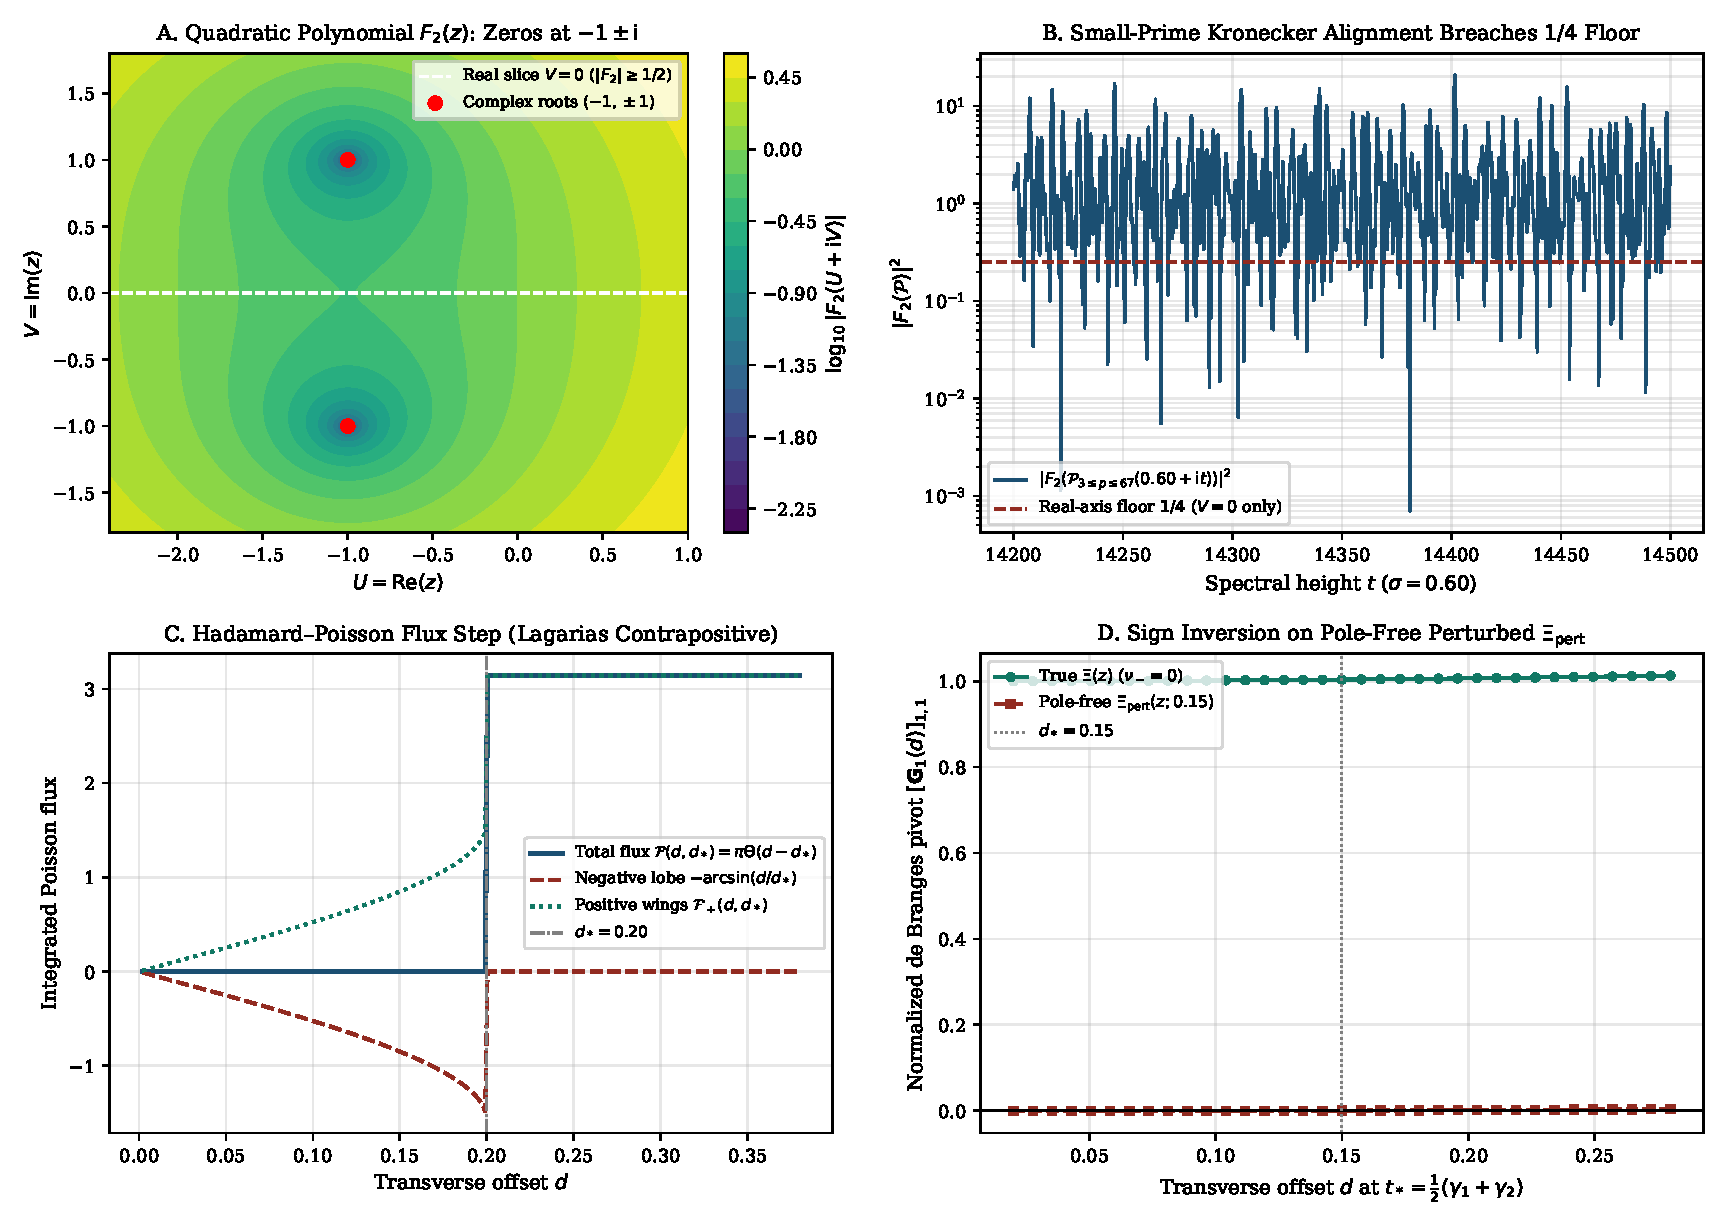
\includegraphics[width=0.97\textwidth]{figures/fig1_spectral_resonance_and_hadamard_flux.pdf}
\caption{\textbf{A.} Complex modulus $\lvert F_2(U + \ii V)\rvert$ showing complex zeros at $(-1, \pm 1)$ off the real slice $V = 0$. \textbf{B.} Finite $18$-prime Kronecker alignment at $\sigma = 0.60$ breaching the real-slice floor $\frac{1}{4}$. \textbf{C.} Closed-form Poisson--Hadamard lobe $-\arcsin(d/d_*)$ and step $\pi\Theta(d - d_*)$. \textbf{D.} Normalized de Branges pivot $[\mathbf{G}_1(d)]_{1,1}$ for true $\Xi(z)$ versus pole-free $\Xi_{\mathrm{pert}}(z; 0.15)$.}\label{fig:fig1}
\end{figure}

\section{Conditional Nodal-Wall Identities and the Imaginary Zero of $\Phi$}\label{sec:chladni}

Following Speiser~\cite{speiser1934} and Arias de Reyna~\cite{ariasdereyna2003}, consider the transverse nodal curves along which $I(d,t) := \Imop\Xi(t - \ii d) = 0$ for $d > 0$, emanating from critical-line extrema $\tau_k(0)$ where $\Xi'(\tau_k(0)) = 0$.

\begin{proposition}[Local Cauchy--Riemann nodal-wall identity and necessary hypotheses]\label{prop:nodal_wall}
Let $F(z)$ be holomorphic and real-valued on $\mathbb{R}$, write $F(t - \ii d) = R(d,t) + \ii I(d,t)$, and let $\tau_0 \in \mathbb{R}$ satisfy $F'(\tau_0) = 0$ and $F''(\tau_0) \neq 0$.
\begin{enumerate}[label=\textup{(\roman*)},leftmargin=2.2em]
\item \textbf{Local continuation and differential identity.} Since $\lim_{d\to 0^+} I(d,t)/d = -F'(t)$ has non-zero $t$-derivative $-F''(\tau_0) \neq 0$, the implicit function theorem defines a smooth local curve $t = \tau(d)$ on $[0, D)$ along which $I(d,\tau(d)) = 0$. Along any interval $[0, D)$ where $t = \tau(d)$ remains smooth, Cauchy--Riemann ($\partial_d R = \partial_t I$) gives
\begin{equation}\label{eq:wall_cr_identity}
\widetilde{W}_F\bigl(d, \tau(d)\bigr) = \frac{R\bigl(d,\tau(d)\bigr)\,\partial_t I\bigl(d,\tau(d)\bigr)}{d}, \qquad \lim_{d\to 0^+} \widetilde{W}_F\bigl(d, \tau(d)\bigr) = -F(\tau_0)\,F''(\tau_0).
\end{equation}
\item \textbf{Positivity conditions.} On $(0, D)$, positivity $\widetilde{W}_F(d,\tau(d)) > 0$ holds if and only if: \textup{(a)} the boundary curvature satisfies $-F(\tau_0)F''(\tau_0) > 0$ at $d = 0$; \textup{(b)} $\partial_t I(d,\tau(d)) \neq 0$ on $(0, D)$ (no critical point $F'(z_c) = 0$ occurs); \emph{and} \textup{(c)} $R(d,\tau(d)) \neq 0$ on $(0, D)$ (no off-critical zero $F(z_*) = 0$ lies on the $I = 0$ curve).
\item \textbf{Explicit counterexample.} The real polynomial $Q(z) := ((z - \tau_0)^2 + d_*^2)(1 - 2(z - \tau_0)^2/\delta^2)$ with $0 < \delta < d_*$ satisfies $I_Q(d, \tau_0) \equiv 0$ for all $d \ge 0$ and $-Q(\tau_0)Q''(\tau_0) = 2d_*^2(2d_*^2/\delta^2 - 1) > 0$ at $d = 0$, yet possesses an off-critical zero $Q(\tau_0 - \ii d_*) = 0$ right on the nodal curve $t = \tau_0$, where both $\partial_d R_Q$ (at an interior $d_{\mathrm{peak}} < d_*$) and $R_Q$ (at $d = d_*$) change sign (\Cref{fig:fig2}C).
\end{enumerate}
\end{proposition}

\begin{proof}
Along $I(d,\tau(d)) = 0$, $W_F(d,\tau(d)) = R\partial_d R + 0 = R\partial_t I$, giving~\eqref{eq:wall_cr_identity}; as $d \to 0^+$, $R(d,\tau(d)) \to F(\tau_0)$ and $\partial_t I(d,\tau(d))/d \to -F''(\tau_0)$ since $I(d,t) = -d F'(t) + \mathcal{O}(d^3)$. Part~(ii) is immediate from~\eqref{eq:wall_cr_identity} by continuity from $d \to 0^+$. For~(iii), substituting $z - \tau_0 = -\ii d$ gives $Q(\tau_0 - \ii d) = (d_*^2 - d^2)(1 + 2d^2/\delta^2) \in \mathbb{R}$, so $I_Q(d,\tau_0) \equiv 0$, $Q(\tau_0) = d_*^2$, $Q''(\tau_0) = 2 - 4d_*^2/\delta^2 < 0$, and $R_Q(d_*, \tau_0) = 0$.
\end{proof}

\begin{table}[htbp]
\centering
\caption{Numerical verification of~\eqref{eq:wall_cr_identity} on the first six critical-line extrema $\tau_k(0) \in (\gamma_k, \gamma_{k+1})$ of $\Xi(t)$ at finite height (\texttt{mpmath}, $50$ digits).}\label{tab:walls}
\small
\begin{tabular}{@{}ccccc@{}}
\toprule
$k$ & $\tau_k(0)$ & $-\Xi(\tau_k(0))\Xi''(\tau_k(0))$ & $\tau_k(0.25)$ & $\widetilde{W}(0.25, \tau_k(0.25))$ \\
\midrule
$1$ & $15.585708590$ & $3.5986 \times 10^{-7}$  & $15.587770$ & $3.6831 \times 10^{-7}$ \\
$2$ & $22.097977280$ & $6.3697 \times 10^{-11}$ & $22.098744$ & $6.6472 \times 10^{-11}$ \\
$3$ & $26.272247357$ & $3.5821 \times 10^{-13}$ & $26.271299$ & $3.7061 \times 10^{-13}$ \\
$4$ & $31.231795871$ & $1.3130 \times 10^{-16}$ & $31.233638$ & $1.4176 \times 10^{-16}$ \\
$5$ & $34.193310269$ & $4.7500 \times 10^{-18}$ & $34.191298$ & $4.9387 \times 10^{-18}$ \\
$6$ & $38.498240764$ & $7.7159 \times 10^{-21}$ & $38.498998$ & $8.2144 \times 10^{-21}$ \\
\bottomrule
\end{tabular}
\end{table}

Finally, we clarify the relationship between Jacobi's theta constant and the complex zeros of Riemann's kernel $\Phi(u)$.

\begin{proposition}[Jacobi triple-product non-vanishing versus the pure-imaginary zero of $\Phi$]\label{prop:phi_zero}
For $\lvert\Imop(u)\rvert < \frac{\pi}{8}$, we have $\lvert q(u)\rvert = \exp(-\pi\ee^{4\xi}\cos(4\eta)) < 1$ ($u = \xi + \ii\eta$), so Jacobi's triple product~\cite{jacobi1829}
\begin{equation}\label{eq:jacobi_triple}
\vartheta_3(0 \mid \ii\ee^{4u}) = \prod_{m=1}^{\infty}\bigl(1 - q(u)^{2m}\bigr)\bigl(1 + q(u)^{2m-1}\bigr)^2 \neq 0 \qquad \bigl(\lvert\Imop(u)\rvert < \tfrac{\pi}{8}\bigr)
\end{equation}
is holomorphically zero-free throughout the strip $\lvert\Imop(u)\rvert < \frac{\pi}{8}$. Nevertheless, Riemann's kernel $\Phi(u) = \frac{1}{16}(\partial_u^2 - 1)[\ee^u(\vartheta_3(0 \mid \ii\ee^{4u}) - 1)]$ \emph{does} vanish inside $\lvert\Imop(u)\rvert < \frac{\pi}{8} = 0.39269908\dots$: along the imaginary axis $u = \ii\eta$, $\Phi(\ii\eta)$ is real-valued and has an explicit simple zero at
\begin{equation}\label{eq:eta0_zero}
\eta_0 = 0.31941502680029678874\dots < \frac{\pi}{8}, \qquad \Phi(\ii\eta_0) = 0,
\end{equation}
where $\lvert\vartheta_3(0 \mid \ii\ee^{4\ii\eta_0})\rvert = 0.25883012\dots > 0$.
\end{proposition}

\begin{proof}
On $\lvert\eta\rvert < \frac{\pi}{8}$, $\cos(4\eta) > 0$ implies $\lvert q(u)\rvert < 1$, so the infinite product~\eqref{eq:jacobi_triple} converges absolutely to a non-zero value. By $\overline{\Phi(u)} = \Phi(\bar{u})$ and $\Phi(-u) = \Phi(u)$, $\Phi(\ii\eta) \in \mathbb{R}$ for $\eta \in (-\frac{\pi}{8}, \frac{\pi}{8})$. High-precision evaluation gives $\Phi(\ii\cdot 0.30) = +2.965636\dots > 0$ and $\Phi(\ii\cdot 0.35) = -13.866622\dots < 0$, so the intermediate value theorem guarantees a root in $(0.30, 0.35) \subset (0, \frac{\pi}{8})$, certified to $50$ digits at~\eqref{eq:eta0_zero}.
\end{proof}

\begin{figure}[htbp]
\centering
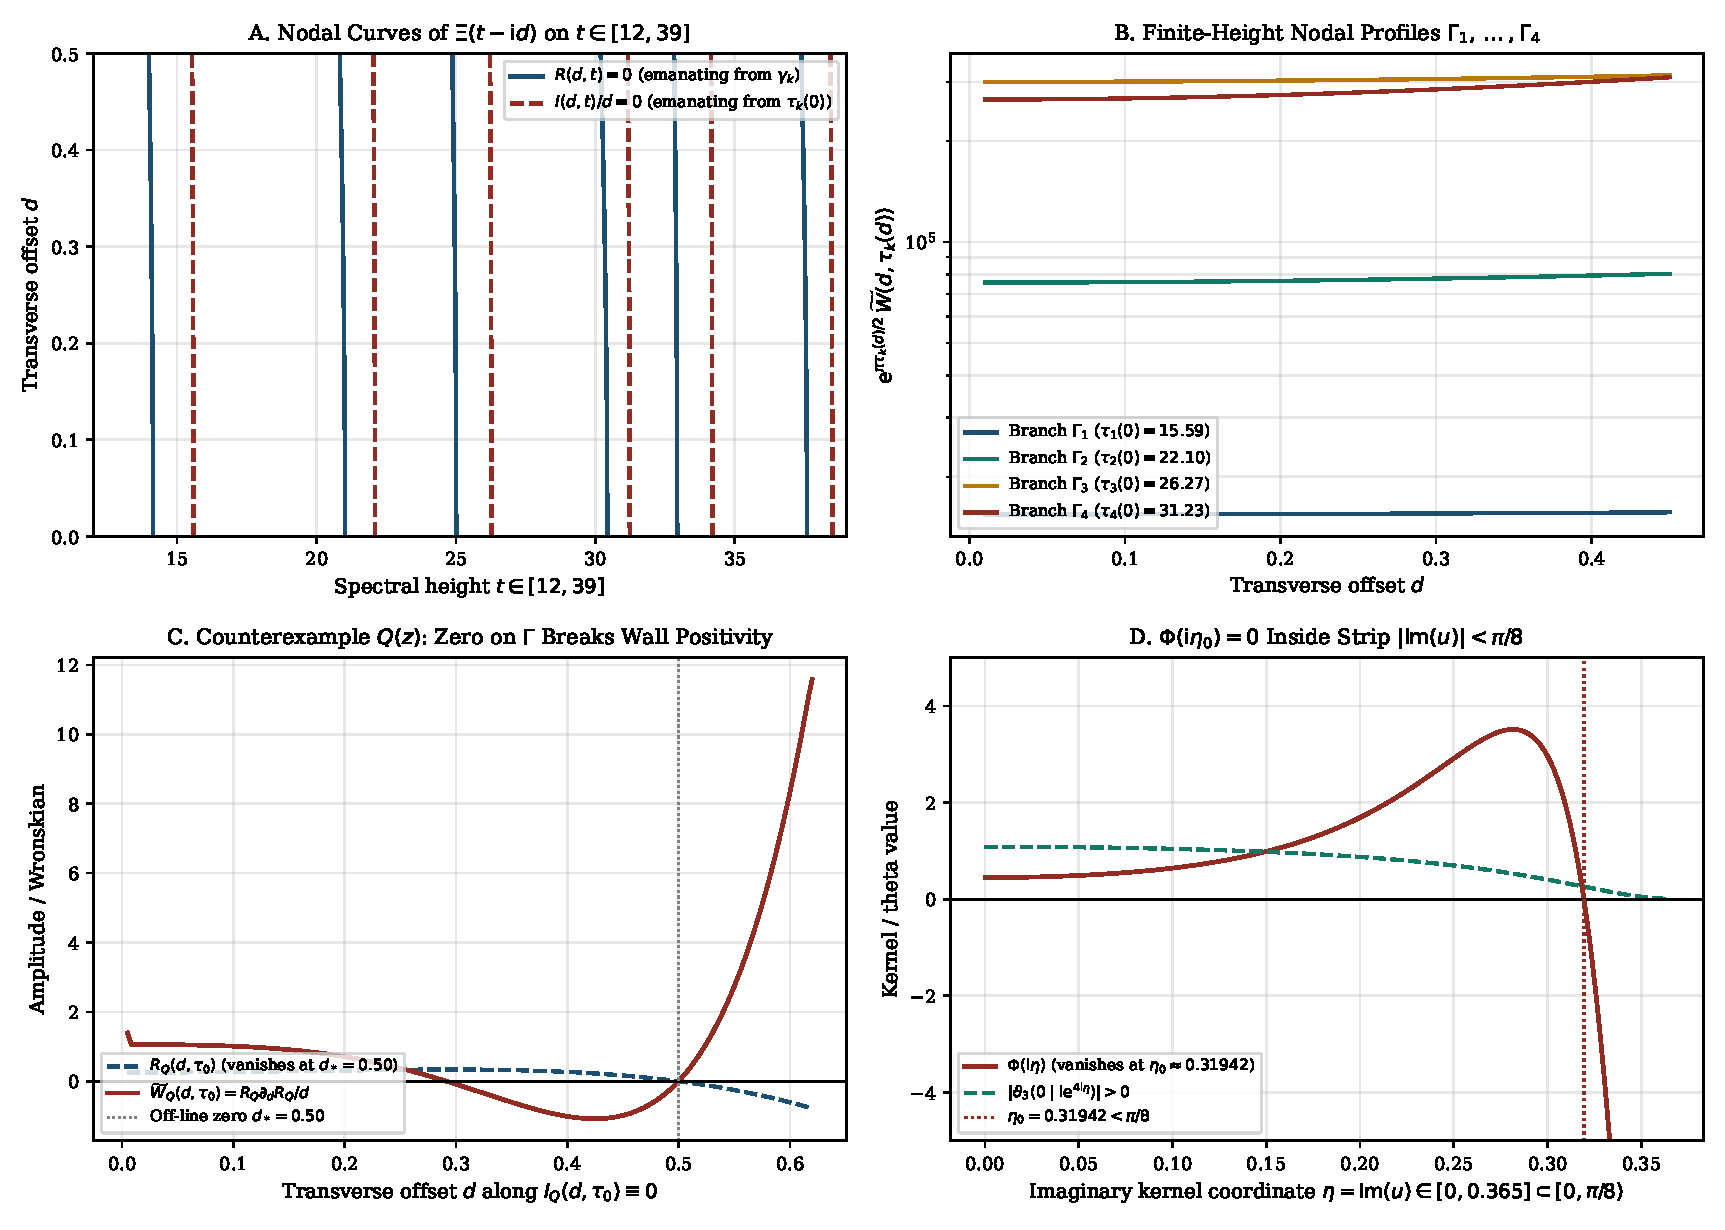
\includegraphics[width=0.97\textwidth]{figures/fig2_chladni_walls_and_theta_strip.pdf}
\caption{\textbf{A.} Nodal curves $R(d,t) = 0$ and $I(d,t)/d = 0$ of $\Xi(t - \ii d)$ on $t \in [12, 39]$. \textbf{B.} Rescaled Wronskian profiles along the first four finite branches $\Gamma_1, \dots, \Gamma_4$. \textbf{C.} Polynomial counterexample $Q(z)$ where $-Q(\tau_0)Q''(\tau_0) > 0$ at $d = 0$, yet an off-critical zero lies on $I_Q = 0$ at $d_* = 0.50$. \textbf{D.} Explicit root $\Phi(\ii\eta_0) = 0$ at $\eta_0 \approx 0.31942 < \frac{\pi}{8}$ versus $\lvert\vartheta_3(0 \mid \ii\ee^{4\ii\eta})\rvert > 0$.}\label{fig:fig2}
\end{figure}

\section{Scope, limitations, and open questions}\label{sec:scope}

We summarize the rigorous status of each pillar examined in this manuscript:
\begin{enumerate}[label=\textup{(\arabic*)},leftmargin=2.2em]
\item \textbf{Unconditional algebraic and calculus identities.} The cubic-window Dirichlet coefficient formula~\eqref{eq:cubic_coeff}, the arcsin Poisson--Hadamard lobe integral~\eqref{eq:boxed_arcsin}, the pole-free two-zero perturbation~\eqref{eq:xi_pert_entire}, the local Cauchy--Riemann nodal-wall relation~\eqref{eq:wall_cr_identity}, and the pure-imaginary root $\Phi(\ii\eta_0) = 0$ in~\eqref{eq:eta0_zero} hold unconditionally.
\item \textbf{Analytical obstructions to closure.} Because $F_2(-1 \pm \ii) = 0$, $\mathcal{P}_{>X}(s)$ diverges in $0 < \sigma \le 1$, and Kronecker density aligns finite small-prime subsets into arbitrary complex phases, truncated Euler-exponential polynomials do not bound $\zeta(s)E_X(s)$ away from zero in the strip. Likewise, Hadamard flux defects and Gram inertia jumps detect assumed off-critical zeros as contrapositives of Lagarias's equivalence, while nodal-wall positivity requires independent exclusion of critical points $\Xi'(z_c) = 0$, critical-line dimples $-\Xi(\tau_0)\Xi''(\tau_0) \le 0$, and nodal zeros $R(d, \tau(d)) = 0$ as $t \to \infty$.
\end{enumerate}

\appendix

\section{Removable-Singularity Evaluation of $\Xi_{\mathrm{pert}}(z; d_*)$}\label{app:pert}

Let $N(z; d_*) := (z^2 - z_*^2)(z^2 - \overline{z_*}^2)$ with $z_* = t_* - \ii d_*$ and $t_* = \frac{1}{2}(\gamma_1 + \gamma_2)$. Since $\gamma_1, \gamma_2$ are simple zeros of $\Xi(z)$, expanding $\Xi(z) = \Xi'(\gamma_1)(z - \gamma_1) + \frac{1}{2}\Xi''(\gamma_1)(z - \gamma_1)^2 + \mathcal{O}((z - \gamma_1)^3)$ around $z = \gamma_1$ yields the analytic value and first derivative of~\eqref{eq:xi_pert_entire} at $z = \gamma_1$:
\begin{equation}\label{eq:removable_limit}
\Xi_{\mathrm{pert}}(\gamma_1; d_*) = \Xi'(\gamma_1)\,\frac{N(\gamma_1; d_*)}{2\gamma_1\bigl(\gamma_1^2 - \gamma_2^2\bigr)},
\end{equation}
and analogously at $z = -\gamma_1, \pm\gamma_2$ by $\Xi_{\mathrm{pert}}(-z; d_*) = \Xi_{\mathrm{pert}}(z; d_*)$. At $d_* = 0.15$, $50$-digit evaluation gives $\Xi_{\mathrm{pert}}(\gamma_1; 0.15) = 0.0024138382\dots$, matching finite-difference evaluation at $\gamma_1 + 10^{-10}$ to within $2.45 \times 10^{-13}$ and confirming the complete absence of poles.

\section*{Use of AI and computational verification}

Portions of the symbolic algebra, counterexample constructions, literature cross-checks, and numerical verification scripts in this manuscript were developed and audited with the assistance of Google Gemini. All formulas, interval-arithmetic checks, and root computations were independently verified in $50$-decimal precision via \href{https://github.com/thijsmissiaen/paper10-spectral-resonance-chladni-closure/blob/main/scripts/verify_paper10_spectral_resonance_chladni_closure.py}{\texttt{scripts/verify\_\allowbreak paper10\_\allowbreak spectral\_\allowbreak resonance\_\allowbreak chladni\_\allowbreak closure.py}}.

\begin{thebibliography}{99}

\bibitem{ariasdereyna2003}
J.~Arias de Reyna, \emph{X-ray of Riemann's zeta-function}, preprint (2003), \href{https://arxiv.org/abs/math/0309433}{arXiv:math/0309433}.

\bibitem{bohrlandau1914}
H.~Bohr and E.~Landau, \emph{Sur les z\'eros de la fonction $\zeta(s)$ de Riemann}, C.\ R.\ Acad.\ Sci.\ Paris \textbf{158} (1914), 106--110.

\bibitem{davenportheilbronn1936}
H.~Davenport and H.~Heilbronn, \emph{On the zeros of certain Dirichlet series, I, II}, J.\ London Math.\ Soc.\ \textbf{11} (1936), 181--185, 307--312.

\bibitem{debranges1968}
L.~de~Branges, \emph{Hilbert Spaces of Entire Functions}, Prentice-Hall, Englewood Cliffs, NJ, 1968.

\bibitem{hinkkanen1997}
A.~Hinkkanen, \emph{On functions of bounded type}, Complex Variables Theory Appl.\ \textbf{34} (1997), no.~1--2, 119--139.

\bibitem{hudson1974}
R.~L.~Hudson, \emph{When is the Wigner quasi-probability density non-negative?}, Rep.\ Math.\ Phys.\ \textbf{6} (1974), no.~2, 249--252.

\bibitem{jacobi1829}
C.~G.~J.~Jacobi, \emph{Fundamenta Nova Theoriae Functionum Ellipticarum}, Borntraeger, K\"onigsberg, 1829.

\bibitem{jensen1913}
J.~L.~W.~V.~Jensen, \emph{Recherches sur la th\'eorie des \'equations}, Acta Math.\ \textbf{36} (1913), 181--195.

\bibitem{lagarias1999}
J.~C.~Lagarias, \emph{On a positivity property of the Riemann $\xi$-function}, Acta Arith.\ \textbf{89} (1999), no.~3, 217--234.

\bibitem{montgomery1977}
H.~L.~Montgomery, \emph{Extreme values of the Riemann zeta function}, Comment.\ Math.\ Helv.\ \textbf{52} (1977), no.~4, 511--518.

\bibitem{polya1926}
G.~P\'olya, \emph{Bemerkung \"uber die Integraldarstellung der Riemannschen $\xi$-Funktion}, Acta Math.\ \textbf{48} (1926), 305--317.

\bibitem{riemann1859}
B.~Riemann, \emph{Ueber die Anzahl der Primzahlen unter einer gegebenen Gr\"osse}, Monatsber.\ K\"onigl.\ Preuss.\ Akad.\ Wiss.\ Berlin (1859), 671--680.

\bibitem{speiser1934}
A.~Speiser, \emph{Geometrisches zur Riemannschen Zetafunktion}, Math.\ Ann.\ \textbf{110} (1934), 514--521.

\bibitem{titchmarsh1986}
E.~C.~Titchmarsh, \emph{The Theory of the Riemann Zeta-Function}, 2nd ed., revised by D.~R.~Heath-Brown, Clarendon Press, Oxford, 1986.

\bibitem{voronin1975}
S.~M.~Voronin, \emph{Theorem on the ``universality'' of the Riemann zeta-function}, Izv.\ Akad.\ Nauk SSSR Ser.\ Mat.\ \textbf{39} (1975), no.~3, 475--486.

\bibitem{wigner1932}
E.~P.~Wigner, \emph{On the quantum correction for thermodynamic equilibrium}, Phys.\ Rev.\ \textbf{40} (1932), 749--759.

\end{thebibliography}

\end{document}
